\documentclass[cn,11pt]{elegantbook}

\title{luodaxiao第五学期笔记}
\subtitle{全文采用Elegant\LaTeX{}模板}

\author{luodaxiao}
\institute{luodaxiao}
\date{\today}
\version{1.0}

\extrainfo{Victory won\rq t come to us unless we go to it. --- M. Moore}

\logo{logo.png}
\cover{cover.jpg}



\begin{document}

\maketitle
\tableofcontents

% \thispagestyle{empty}

\mainmatter
\hypersetup{pageanchor=true}

\chapter{嵌入式系统设计}

\large{此复习试题主要为个人\textbf{(luodaxiao)}使用,不能确保结果的正确性,也不能保证是否会考这些题,大家慎用.}
\section{需要掌握的题}

\subsection{重点强调,考试时必考但有所变化}
	\begin{figure}[htbp]
	\centering
	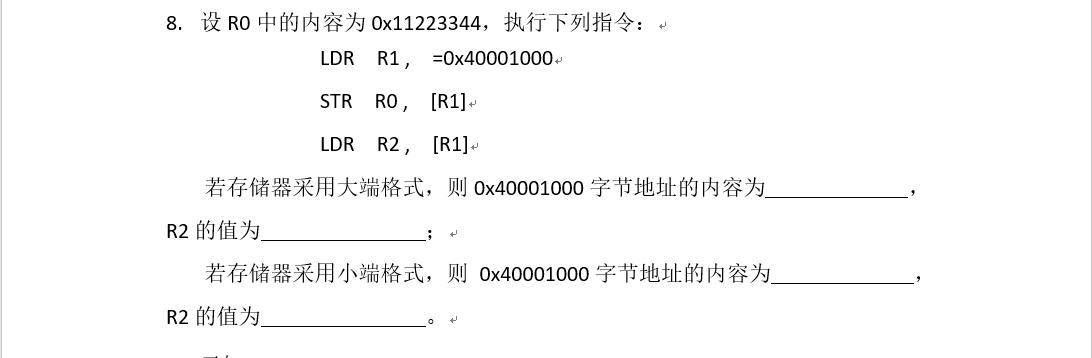
\includegraphics[height=6.0cm,width=15cm]{image/8.png}%figures文件夹下的DSC.png图片,
	\caption{嵌入式系统的组成}
\end{figure}

	\begin{figure}[htbp]
	\centering
	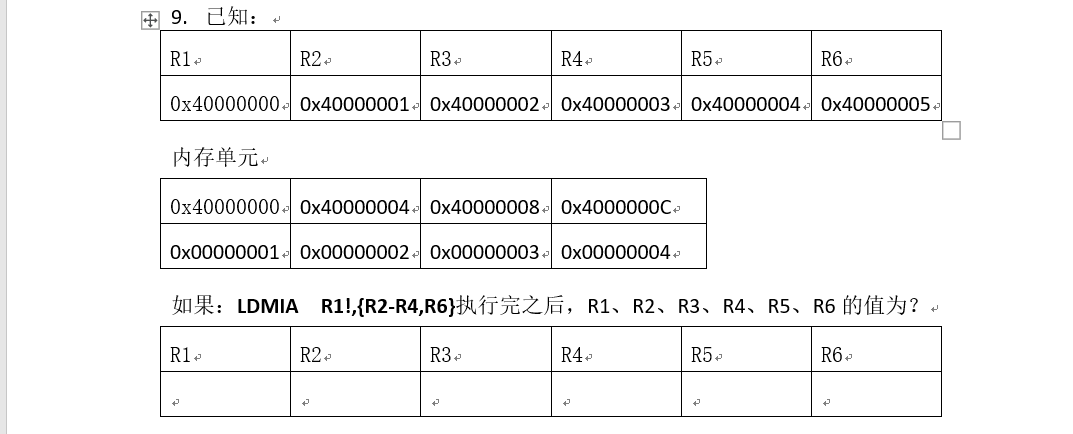
\includegraphics[height=6.0cm,width=15cm]{image/9.png}%figures文件夹下的DSC.png图片,
	\caption{嵌入式系统的组成}
\end{figure}
\subsection{嵌入式系统的定义}
嵌入到对象体系中的专用计算机应用系统.
\subsection{特点}
\begin{lstlisting}
特点:
1. 嵌入性
2. 内含计算机 
3. 专用性
\end{lstlisting}


\subsection{嵌入式系统的组成}
	\begin{figure}[htbp]
	\centering
	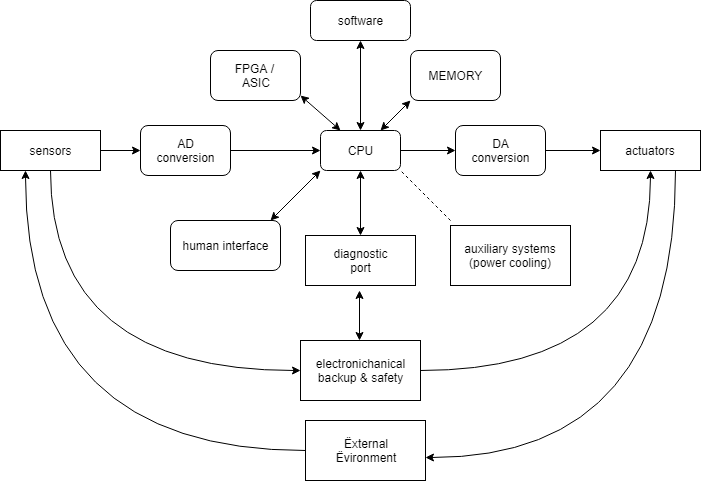
\includegraphics[height=6.0cm,width=9.5cm]{image/qianrushizucheng.png}%figures文件夹下的DSC.png图片,
	\caption{嵌入式系统的组成}
\end{figure}
\subsection{LPC系列含有哪些外设(至少答5个)}
外部中断、捕获/比较定时器0/1、ADC、通用I/O、PWM0、实时时钟、$I^2$C串行接口、SPI串行接口、
UAR10$\&$1、看门狗定时器、系统控制、PLL、译码器、外部存储器控制器

\subsection{ARM的处理器状态与工作模式}
状态:ARM、Thumb
\begin{lstlisting}
工作模式(7种):
	1.用户模式
	2.系统模式
	3.快中断模式
	4.中断模式
	5.管理模式
	6.中止模式
	7.未定义模式
\end{lstlisting}
除用户模式和系统模式外,均为异常模式。究竟如何进入异常模式,具体规定如下:
\begin{lstlisting}
	* 处理器复位之后进入管理模式,操作系统内核通常处于管理模式;
	* 当处理器访问存储器失败时,进入数据访问终止模式;
	* 当处理器遇到不支持的指令时,进入未定义模式;
	* 中断模式与快中断模式分别对ARM处理器两种不同级别的中断作出响应.
\end{lstlisting}

\subsection{ARM异常及其入口地址}
\begin{lstlisting}
	 地址			    	异常
	0x00000000			复位
	0x00000004			未定义指令
	0x00000008			软件中断
	0x0000000c			预取指中止
	0x00000010			数据中止
	0x00000014			保留*
	0x00000018			IRQ
	0x0000001c			FIQ
\end{lstlisting}
\subsection{复位时是什么状态?}
选择题:ARM状态


\subsection{LPC包含哪四大部分?}
\begin{lstlisting}
1.CPU
2.存储器
3.AHB总线外设
4.VPB总线外设
\end{lstlisting}
\subsection{VPB总线上挂接了哪些外设?}
外部中断、捕获/比较定时器0/1、ADC、通用I/O、PWM0、实时时钟、$I^2$C串行接口、SPI串行接口、
UAR10$\&$1、看门狗定时器、系统控制
\subsection{Flash编程的3种方法}

\begin{lstlisting}
1.使用JTAG仿真/调试器,通过芯片的JTAG接口下载程序;
2.使用在系统编程(ISP),通过UART0接口下载程序;
3.使用在应用编程(IAP).
\end{lstlisting}


\subsection{系统控制模块包含哪些部分?}
晶体振荡器、复位、存储器映射器、锁相环(PLL)、VPB分频器、功率控制、唤醒定时器
\subsection{画出阻容复位电路,并解释各元件的工作原理}
阻容复位电路图略.

当上电时,由于电容C两端电压不能突变,C极两端电压经过一段时间充电逐渐上升,直至达到电源电压;当无外加电源时,通过二极管D1迅速放电,以确保下次上电时能及时复位.二极管的作用:产生快速放电的通路.
\subsection{最小系统是什么?它包含哪些部分?}
\begin{lstlisting}
	CPU及提供CPU运行的外设电路所组成的系统叫做嵌入式的最小系统.
\end{lstlisting}
\begin{lstlisting}
最小系统包括:
			1.CPU 2.存储器 3.复位及复位控制 4.电源 5.时钟
\end{lstlisting}

\subsection{如何降低系统的功耗?(第19题)}
\begin{lstlisting}
	从硬件方面:
1.降低系统时钟频率		2.使用多电压兼容系统			3.工艺改进促使低电压供电
4.选用低功耗的CPU		  5.选用低功耗的存储器		  6.选用高速低频的工作方式

	从软件方面:
1.编译低功耗优化技术		   2.采用更快速的算法			3.通信系统提高通信波特率
4.采集系统尽量降低采集速率	5.静态显示				     6.睡眠方式
7.软件设计成中断驱动方式	 8.硬件软件化				 9.尽量减少处理器运行时间
\end{lstlisting}
\begin{note}
本题问的是降低系统功耗,需从两个方面回答,一方面是软件另一方面则为硬件,两方面至少各答五条
\end{note}



\section{英文题}
考虑到有一题为英文题,故做了一下笔记:
\begin{lstlisting}
RISC:精简指令集计算机         CISC:复杂指令集计算机
RTOS:实时操作系统(real-time opration-system)
Core:内核						task:任务
ISR:中断服务				  schedule:调度
SP:堆栈指针(stack pointer)    FILO:先进后出(first in last out)
EMPU:嵌入式微处理器			ALU:算术逻辑单元
MCP:微控制器				   CPSR:程序状态寄存器
SoC:片上系统				   SPSR:程序状态保存寄存器
ADC:模数转换器				 PWM:脉冲宽度调制
ISP:在系统编程				  IAP:在应用编程技术
PLL:锁相环						MISO:主入从出
MOSI:主出入					VIC:向量中断控制器
SCK:串行时钟
\end{lstlisting}


\begin{remark}
	江西理工大学 \lstinline{ARM嵌入式操作系统基础教程}      不需要掌握每个单词的拼写,记住\lstinline{单词缩写}即可.

\end{remark}


\chapter{电子电路设计}
\subsection{ADC}

\subsection{开关电路}










\end{document}
